\section{Электромагнитные волны в однородных, изотропных диэлектрических средах. Уравнения Максвелла. Поперечность электромагнитной волны. Взаимная
ориентация волнового вектора, векторов электрического и магнитного полей в
плоской волне. Стоячие электромагнитные волны. Опыты Винера.}
\noindent\rule{\textwidth}{0.5pt}

\subsection{Ликбез}

\textbf{Изотропной} среда называется если её физические свойства ($\epsilon$, $\mu$, $\sigma$ и другие) не зависят от направления\\ \\
\textbf{Электромагнитной} волна называется потому что характеризуется двумя взаимно ортогональными векторами: \textbf{E} и \textbf{H} - векторами напряженности электрического и магнитного полей, в процессе колебаний электрическое поле постепенно переходит в магнитное, магнитное — в электрическое.\\ \\
\textbf{Фронтом} волны называют поверхность, до которой дошёл волновой процесс к данному моменту времени. По форме волнового фронта выделяют простейшие волны: сферическую, плоскую, цилиндрическую. Нормаль к волновому фронту совпадает с направлением распространения волны в данной точке.\\ \\
\textbf{Плоская волна} - волна, фронт у которой плоский (движущиеся в пространстве параллельные плоскости).\\ \\
\textbf{Волновой вектор} - вектор, направление которого перпендикулярно фазовому фронту бегущей волны, а абсолютное значение равно волновому числу.\\ \\
\textbf{Волновое число} - отношение $2 \pi$ радиан к длине волны\\ \\
Исходной системой для определения электромагнитного поля в среде является система \textbf{уравнений Максвелла}:
\\
\begin{spacing}{0.7}
$$ rot  \textbf{H} = \frac{1}{c} \frac{\partial \textbf{D}}{\partial t} + 
\frac{4\pi}{c} \textbf{j}, \eqno{(1)}$$
\\
$$ rot \textbf{E} = -\frac{1}{c} \frac{\partial \textbf{B}}{\partial t},\eqno{(2)} $$
\\
$$ div \textbf{D} = 4 \pi \rho, \eqno{(3)} $$
\\
$$ div \textbf{B} = 0. \eqno{(4)}  $$\\

\end{spacing}

Здесь \textbf{E} и \textbf{H} - напряженности электрического и магнитного полей, \textbf{B} и \textbf{D} - векторы электрической и магнитной индукции, $\textbf{j}$ и $\rho$ - плотности токов и электрических зарядов в среде, их появление связано с действием электромагнитного поля, между собой они связаны уравнением непрерывности:

$$ div \textbf{j} + \frac{\partial \rho}{\partial t} = 0, \eqno{(5)}$$ 

Оно отражает закон сохранения полного электрического заряда внутри объема среды.\\ 
Уравнение (3) является следствием уравнений (1) и (5) (дивергенция от обоих частей (1), использование (5)), а (4) может быть получено из (2) (дивергенция от обоих частей (2), $div \ rot E = 0$), поэтому 
система уравнений (1) - (5) не является полной и для её решения относительно \textbf{E}, \textbf{H}, \textbf{B}, \textbf{D} и \textbf{j} надо дополнить систему тремя материальными уравнениями:

$$  \textbf{D} = \textbf{D}(\textbf{E}), \ \textbf{B}=\textbf{B}(\textbf{H}), \  \textbf{j = \textbf{j}}(\textbf{E})$$

Для однородной изотропной среды с диэлектрической проницаемостью $\epsilon$, магнитной проницаемостью $\mu$ и удельной проводимостью $\sigma$ эти уравнения принимают вид:

$$  \textbf{D} = \epsilon (\textbf{E}),  \textbf{B} = \mu (\textbf{H}), \textbf{j} = \sigma (\textbf{E})$$

\subsection{Уравнения Максвелла}

Для диэлектрической среды $\sigma = 0$ уравнения Максвелла перепишутся в виде:

\begin{spacing}{0.7}
$$ rot  \textbf{H} = \frac{\epsilon}{c} \frac{\partial \textbf{E}}{\partial t}, $$
\\
$$ rot \textbf{E} = -\frac{\mu}{c} \frac{\partial \textbf{H}}{\partial t}, $$
\\
$$ div \textbf{E} = 0,  $$
\\
$$ div \textbf{H} = 0. $$
\end{spacing}

\subsection{Электромагнитные волны в однородных, изотропных диэлектрических средах}

Исключая из системы \textbf{H} ($rot \ rot \textbf{E}  = grad \ div \textbf{E} - \nabla^2 \textbf{E}  = - \nabla^2 \textbf{E},$ получим уравнение на вектор \textbf{E}: 

$$ {\nabla}^2\textbf{E} - \frac{\epsilon \mu}{c^2} \frac{{\partial}^2 \textbf{E}}{\partial t^2} = 0$$

И такое же на \textbf{H}:

$$ \ {\nabla}^2\textbf{H} - \frac{\epsilon \mu}{c^2} \frac{{\partial}^2 \textbf{H}}{\partial t^2} = 0$$

Если искать решения данных уравнений в виде монохроматических (строго гармонических волн с постоянной во времени частотой, амплитудой и начальной фазой) волн, то получаем:

$$ {\nabla}^2\textbf{E} + k^2 \textbf{E} = 0, \ \ \ {\nabla}^2\textbf{H} + k^2 \textbf{H} = 0, \ \ \ k = \frac{\omega}{c}\sqrt{ \epsilon \mu}$$

Здесь $k$ - величина комплексного \textbf {волнового вектора} $\textbf{k} = k \textbf{s},$ где \textbf{s} - единичный вектор в направлении распространения волны. Его удобно представлять в виде $k = k_0(n -ik),$ где $k_0 = \frac{\omega}{c}$, а $n$ и $k$ называются коэффициентами преломления и поглощения соответственно.\\ \\

\subsection{Взаимная ориентация волнового вектора, векторов электрического и магнитного полей в плоской волне}


Эти три вектора образуют правую тройку векторов.

Векторы \textbf{E} и \textbf{H} могут быть представлены в виде:
$$ \textbf{E} = A_1 \exp{(i(\omega t - \textbf{k}\textbf{r}))}, \ \textbf{H} = A_2 \exp{(i(\omega t - \textbf{k}\textbf{r}))}$$
Связь между ними следует из закона электромагнитной индукции Фарадея:
$$ rot \textbf{E} = - i [\textbf{k}, \textbf{E}] = -i\frac{\omega}{c} \sqrt{n^2 + k^2} [\textbf{s}, \textbf{E}] \exp{(-i \arctg{(\frac{k}{n})})}$$
Отсюда:
$$ \textbf{B} = \sqrt{n^2 + k^2}[\textbf{s}, \textbf{E}] \exp{(-i \arctg{(\frac{k}{n})})}$$


\subsection{Поперечность электромагнитной волны}

Чтобы определить структуру волн, а именно доказать их \textbf{поперечность} перейдём к рассмотрению поля в котором векторы \textbf{E} и \textbf{H} зависят от одной пространственной координаты $\xi = (\textbf{m}\textbf{r})$ ($+m$ - направление распространения волны) и времени $t$, тогда:

$$ div \textbf{E} = \frac{\partial}{\partial \xi} (\textbf{m}\textbf{E}),
\ \ \ rot \textbf{E} = \frac{\partial}{\partial \xi}[\textbf{m}\textbf{E}],$$
Уравнения Максвелла для такой системы:

$$\frac{\partial}{\partial \xi}[\textbf{m}\textbf{H}] = \frac{\epsilon}{c} \frac{\partial \textbf{E}}{\partial t},$$

$$\frac{\partial}{\partial \xi}[\textbf{m}\textbf{E}] = -\frac{\mu}{c} \frac{\partial \textbf{H}}{\partial t},$$ 

$$\frac{\partial}{\partial \xi} (\textbf{m}\textbf{E}) = \frac{\partial \textbf{E}_\xi}{\partial \xi} = 0$$

$$\frac{\partial}{\partial \xi} (\textbf{m}\textbf{H}) = \frac{\partial \textbf{H}_\xi}{\partial \xi}  = 0$$
\\ \\
Значит, проекции векторов  \textbf{E} $\textbf{E}_\xi $ и \textbf{H} $\textbf{H}_\xi $ на направление распространения волны могут зависить только от времени. Умножая первые два уравнения скалярно на \textbf{m}, получаем:
$$ \frac{\partial \textbf{E}_\xi}{\partial t} = \frac{\partial \textbf{H}_\xi}{\partial t} = 0$$
Т.е. проекции не зависят так же и от времени, что означает что электромагнитные волны в диэлектрической среде являются поперечными волнами, векторы \textbf{E} и \textbf{H} лежат в плоскости фронта волны.\\ \\

\subsection{Стоячая волна}

\textbf{Стоячая волна} есть результат суперпозиции двух электромагнитных волн бегущих навстречу друг другу:

Если первая волна распространяется в положительном направлении оси x и задается: $$E_y = E_m \cos{(\omega t - kx)},\ \ H_z = H_m \cos{(\omega t - kx)},$$ то уравнение волны бегущей в обратном направлении получается если заменить в скобках минусы на плюсы, учитывая что векторы \textbf{E}, \textbf{H}, \textbf{k} должны составлять правую тройку. Уравнение встречной:
$$E_y = E_m \cos{(\omega t + kx)}, \ \ H_z = -H_m \cos{(\omega t + kx)}$$

Результирующая:
$$E_y = 2E_m \cos{(kx)}\cos{(\omega t)}, \ \ H_z = 2H_m \sin{(kx)}\sin{\omega t)}$$

Колебания векторов \textbf{E}, \textbf{H} сдвинуты по фазе на $\pi/2$, для амплитудных значений $E_m$ и $H_m$ выполняется соотношение:

$$E_m \sqrt{\epsilon \epsilon_0} = H_m \sqrt{\mu \mu_0}$$

Если в некоторый момент $ E_y$ во всех точках имело максимальное значение и при этом $ H_z =0$, то через четверть периода картина будет обратной: $ H_z$ достигнет всюду максимальных значений со сдвигом в пространстве на $ \lambda/4$, а $ E_y$ обратится в нуль. 
\\ 

\subsection{Опыт Винера}


\begin{figure}[H]
	\centering
	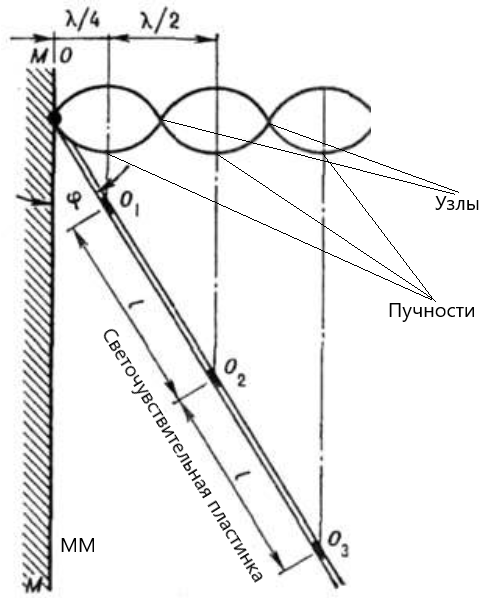
\includegraphics[scale = 0.5]{Viner}
\end{figure}

На плоское металл.зеркало (ММ)  направляется по нормали монохроматич. свет длиной волны  $\lambda$ . При отражении световых волн от этой поверхности образуются стоячие волны, узловые плоскости к-рых параллельны MМ и отстоят друг от друга на расстоянии $\frac{\lambda}{2}$ ; при этом на поверхности находятся узел электрич. вектора (E=0) и пучность магн. вектора. Под малым углом к поверхности зеркала располагается стеклянная пластинка с тонким $\frac{\lambda}{20}$  светочувствит. слоем эмульсии. Светочувствит. слой пересекался с пучностями векторов стоячей волны по прямым, параллельным поверхности зеркала. После  проявления на пластинке возникает система параллельных тёмных полос (O1, O2, O3), соответствующих местам макс. выделения серебра. Винер установил, что первая тёмная полоса располагается не на краю светочувствит. слоя, граничащего с металлич. зеркалом, а отстаёт от него на $\frac{\lambda}{4}$. Именно на этом расстоянии располагается первая пучность (пучность — точка или область в пространстве, в которой амплитуда максимальна и равна сумме амплитуд интерферирующих волн (амплитуда стоячей волны в пучностях вдвое больше амплитуды каждой из интерферирующих волн) электрической световой волны, т. е. фотографическое действие световой волны связано с её электрич. вектором.